\documentclass[12pt,a4paper]{article}

% ── Packages ─────────────────────────────────────────────
\usepackage[T1]{fontenc}
\usepackage[utf8]{inputenc}
\usepackage[margin=2.5cm]{geometry}
\usepackage{booktabs}
\usepackage{array}
\usepackage{tabularx}
\usepackage{longtable}
\usepackage{listings}
\usepackage{xcolor}
\usepackage{hyperref}
\usepackage{fancyhdr}
\usepackage{titlesec}
\usepackage{parskip}
\usepackage{enumitem}
\usepackage{tikz}
\usepackage{caption}
\usepackage{amsmath}
\usepackage{graphicx}
\usepackage{float}
\usepackage{placeins}
\usepackage{needspace}

% ── Colors ───────────────────────────────────────────────
\definecolor{codeblue}{RGB}{0,90,160}
\definecolor{codegray}{RGB}{80,80,80}
\definecolor{codegreen}{RGB}{30,130,50}
\definecolor{codebg}{RGB}{248,248,248}
\definecolor{accentblue}{RGB}{0,80,150}
\definecolor{lightgray}{RGB}{230,230,230}

% ── Listings ─────────────────────────────────────────────
\lstset{
backgroundcolor=\color{codebg},
basicstyle=\ttfamily\small,
keywordstyle=\color{codeblue}\bfseries,
commentstyle=\color{codegreen},
numbers=left,
numberstyle=\tiny,
frame=single,
breaklines=true,
captionpos=b,
language=C
}

% ── Header ───────────────────────────────────────────────
\pagestyle{fancy}
\fancyhf{}
\fancyhead[L]{CSE 396 Project}
\fancyhead[R]{MOD-07 Autonomy SW}
\fancyfoot[C]{\thepage}

% ── Title Styles ─────────────────────────────────────────
\titleformat{\section}{\large\bfseries\color{accentblue}}{\thesection.}{0.6em}{}
\titleformat{\subsection}{\normalsize\bfseries}{\thesubsection}{0.5em}{}

% ─────────────────────────────────────────────────────────
\begin{document}

\begin{titlepage}
\centering
\vspace*{2cm}

{\Huge\bfseries MOD-07: Autonomy SW\par}
\vspace{0.5cm}
{\Large Technical Documentation\par}

\vspace{2cm}

\begin{tabular}{ll}
Name 1: & Ayşe Feyza SERBEST \\
Name 2: & Görkem UYSAL \\
Version: & 0.2 \\
Date: & March 29, 2026 \\
\end{tabular}

\vfill
CSE 396 — Autonomous Fire Detection Rover
\end{titlepage}

\tableofcontents
\newpage

% ========================================================
\section{Purpose}

MOD-07 (Autonomy SW) is the central decision-making layer of the Autonomous Fire Detection
and Suppression Rover. It implements a \textbf{Finite State Machine (FSM)} that integrates sensor
data from multiple modules and issues coordinated commands to all actuator subsystems.

No other module contains mission-level logic. All remaining modules are either hardware drivers
or software abstractions over hardware. MOD-07 is the sole component that determines \emph{what
the rover should be doing at any given moment}, making it the architectural apex of the system.

The module's responsibilities are:
\begin{itemize}[leftmargin=1.5em]
    \item Consuming structured flame detection data from MOD-02 (\texttt{flame\_data\_t}).
    \item Consuming real-time proximity data from MOD-05 (\texttt{distance\_cm}).
    \item Transitioning the FSM across seven defined states based on sensor conditions.
    \item Issuing motion commands to MOD-04 (\texttt{motion\_direction\_t}, \texttt{speed}).
    \item Issuing suppression commands to MOD-06 (\texttt{suppression\_cmd\_t}).
    \item Exposing its current state to MOD-08 for testing and validation.
\end{itemize}

% ========================================================
\FloatBarrier
\section{Dependencies}

\begin{table}[H]
\centering
\begin{tabularx}{\linewidth}{llX}
\toprule
Module & Name & Usage \\
\midrule
MOD-02 & Flame Detection & Flame direction / intensity input \\
MOD-04 & Motion Control & Receives movement commands \\
MOD-05 & Distance Sensor & Obstacle / range input \\
MOD-06 & Fire Suppression & Pump activation output \\
MOD-08 & Test Module & FSM verification \\
\bottomrule
\end{tabularx}
\caption{Dependencies of MOD-07}
\end{table}

% ========================================================
\FloatBarrier
\section{FSM Design}

\subsection{State Enumeration}

\begin{lstlisting}[caption={FSM States}]
typedef enum {
STATE_SEARCH,
STATE_DETECT,
STATE_APPROACH,
STATE_AVOID_OBSTACLE,
STATE_STOP,
STATE_EXTINGUISH,
STATE_VERIFY
} autonomy_state_t;
\end{lstlisting}

\subsection{Transition Diagram}

\begin{figure}[H]
\centering
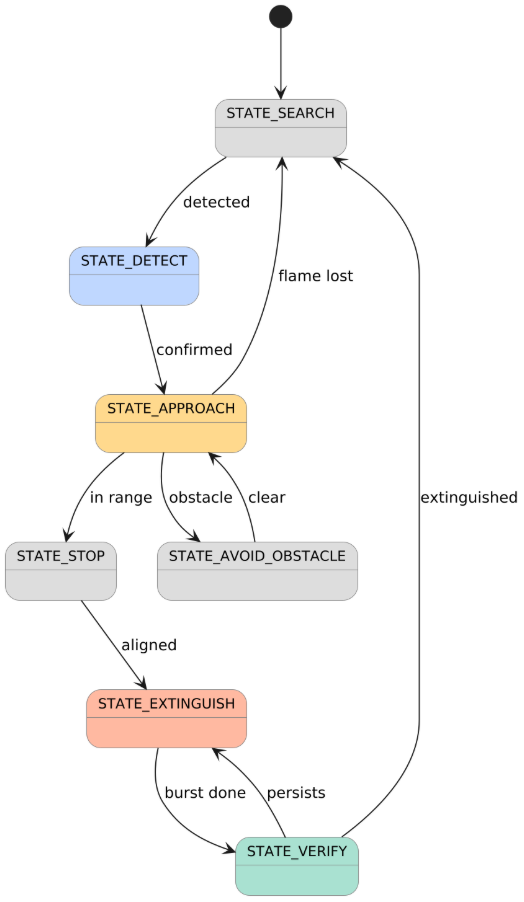
\includegraphics[width=0.52\textwidth]{diagram3.png}
\caption{FSM State Transition Diagram}
\end{figure}

\FloatBarrier
\Needspace{12\baselineskip}
\subsection{State Descriptions}

\begin{table}[H]
\centering
\caption{FSM state descriptions and trigger conditions}
\begin{tabularx}{\linewidth}{llX}
    \toprule
    \textbf{State} & \textbf{Actuators Active} & \textbf{Description \& Exit Condition} \\
    \midrule
    \texttt{STATE\_SEARCH}
        & MOD-04 (rotate)
        & Rover rotates in place, polling MOD-02 continuously.
          Exits when \texttt{flame\_data\_t.detected == true}. \\[4pt]
    \texttt{STATE\_DETECT}
        & None
        & Flame signal confirmed; direction is resolved.
          Exits immediately to \texttt{STATE\_APPROACH} once direction is stable. \\[4pt]
    \texttt{STATE\_APPROACH}
        & MOD-04 (drive)
        & Rover drives toward flame using directional commands.
          MOD-05 is polled every cycle.
          Exits to \texttt{STATE\_STOP} when \texttt{distance\_is\_unsafe()} returns true,
          or to \texttt{STATE\_AVOID\_OBSTACLE} on lateral obstacle detection.
          Exits to \texttt{STATE\_SEARCH} if flame is lost. \\[4pt]
    \texttt{STATE\_AVOID\_OBSTACLE}
        & MOD-04 (steer)
        & Rover executes avoidance maneuver.
          Exits back to \texttt{STATE\_APPROACH} when path is clear. \\[4pt]
    \texttt{STATE\_STOP}
        & None
        & All motors halted; rover aligns with flame.
          Exits to \texttt{STATE\_EXTINGUISH}. \\[4pt]
    \texttt{STATE\_EXTINGUISH}
        & MOD-06 (pump on)
        & Water pump is activated via \texttt{suppression\_cmd\_t}.
          MOD-02 is polled to detect flame extinction.
          Exits to \texttt{STATE\_VERIFY} after pump burst completes. \\[4pt]
    \texttt{STATE\_VERIFY}
        & None
        & Confirms \texttt{flame\_data\_t.detected == false}.
          Exits to \texttt{STATE\_SEARCH} if flame persists;
          exits to \texttt{STATE\_STOP} (idle) if extinguished. \\
    \bottomrule
\end{tabularx}
\end{table}

% ========================================================
\FloatBarrier
\section{Data Types}

\subsection{Input Structure}

\begin{lstlisting}[caption={autonomy_input_t}]
typedef struct {
    flame_data_t flame_data;
    uint16_t distance_cm;
} autonomy_input_t;
\end{lstlisting}

\begin{table}[H]
\centering
\begin{tabularx}{\linewidth}{llX}
\toprule
Field & Type & Description \\
\midrule
flame\_data & flame\_data\_t & Flame direction/intensity data \\
distance\_cm & uint16\_t & Distance in cm \\
\bottomrule
\end{tabularx}
\caption{Input Structure Fields}
\end{table}

\subsection{Output Structure}

\begin{lstlisting}[caption={autonomy_output_t}]
typedef struct {
    motion_direction_t motion_cmd;
    uint8_t speed;
    uint8_t pump_on;
} autonomy_output_t;
\end{lstlisting}

\begin{table}[H]
\centering
\begin{tabularx}{\linewidth}{llX}
\toprule
Field & Type & Description \\
\midrule
motion\_cmd & motion\_direction\_t & Direction command \\
speed & uint8\_t & PWM speed (0-255) \\
pump\_on & uint8\_t & Pump activation flag \\
\bottomrule
\end{tabularx}
\caption{Output Structure Fields}
\end{table}

% ========================================================
\FloatBarrier
\section{API Summary}

\begin{table}[H]
\centering
\begin{tabularx}{\linewidth}{lX}
\toprule
Function & Description \\
\midrule
autonomy\_init() & Initializes FSM \\
autonomy\_update(in) & Updates FSM with sensor input \\
autonomy\_get\_output(out) & Returns current commands \\
autonomy\_reset() & Resets FSM \\
autonomy\_get\_current\_state() & Returns current state \\
\bottomrule
\end{tabularx}
\caption{Public API}
\end{table}

% ========================================================
\FloatBarrier
\section{Operational Flow}

\begin{enumerate}
\item Search for flame
\item Detect target
\item Move toward flame
\item Avoid obstacles if needed
\item Stop at safe distance
\item Activate pump
\item Verify extinguished
\item Return to search mode
\end{enumerate}

% ========================================================
\FloatBarrier
\section{Known Limitations}

\begin{itemize}
\item No advanced path planning
\item No timeout watchdog
\item No speed ramping
\item Sensor noise may affect transitions
\end{itemize}

% ========================================================
\FloatBarrier
\section{Version History}

\begin{table}[H]
\centering
\begin{tabularx}{\linewidth}{llX}
\toprule
Version & Date & Notes \\
\midrule
0.1 & 2026-03-28 & Initial FSM created \\
0.2 & 2026-03-29 & Added new states and robustness \\
\bottomrule
\end{tabularx}
\caption{Version History}
\end{table}

\end{document}